\chapter{Introduction}
\label{chapter:Intro}

Blockchain technology has seen an enormous rise in interest in the recent years, coming to its climax at the end of 2017. This development purportedly mainly driven by the cryptocurrency bitcoin which is the most widely known cryptocurrency in the market and whose value increased from \$900 to \$20.000 within the last year.\footcite[Cf.][]{Higgins900200002017}
However, with the rise in interest, the number of persons wondering \enquote{But what exactly is bitcoin?} and \enquote{What is this blockchain technology?} has also spiked. Simple Google search requests for \enquote{\textit{what is bitcoin}} and \enquote{\textit{what is blockchain}} have peaked in December 2017, as illustrated in figure \ref{fig:SearchRequests}, and yield 10.6 million and 3.8 million results. Of these results, the top ones claim to explain the technology in as little words as possible (\enquote{\textit{WTF is The Blockchain?
The ultimate 3500-word guide in plain English to understand Blockchain.}}\footcite{MamoriaWTFBlockchain2017}, \enquote{\textit{Explain Bitcoin Like I'm 5}}\footcite{CustodioExplainBitcoinFive2013}, \enquote{\textit{Blockchain: everything you want to know about the technology but were too embarrassed to ask}}\footcite{HeathmannBlockchaineverythingyou2018}, or \enquote{\textit{Still don't understand the blockchain? This explainer will help}}\footcite{LeighSinodStilldonunderstand2018}), trying to catch the attention of everyone who has not yet understood this technology. In fact, there are various articles, videos, and further resources available online which all try to explain the technology in an easy to understand manner. However, these claims appear to be empty promises, as most of them do not introduce the learner to the overall value of the technology, but instead explain the technical details behind blockchain. As one expert states, these resources, mostly published by blockchain enthusiasts, \enquote{are too technical [..] and missing the \textit{easy} language},\footcite[Cf.][P19, P20]{DanielKaltenbach_Interview} thus discouraging people with little or no knowledge from learning more about the technology.

\begin{figure}
    \centering
    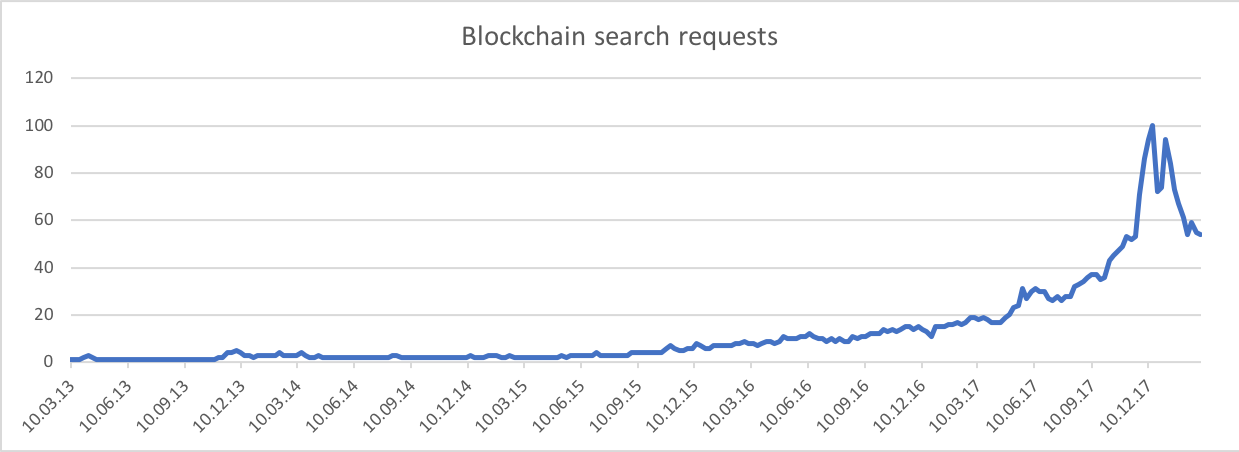
\includegraphics[width=\textwidth]{latex-vorlage_v1.5/graphics/BCRQ.png}
    \caption[Google Trends results for \enquote{blockchain} search requests.]{Google Trends results for \enquote{blockchain} search requests.\protect\footnotemark}
    \label{fig:SearchRequests}
\end{figure}
\footnotetext{Data extracted on the 12th of march, 2018 from https://trends.google.com/trends/explore?date=today\%205-y\&q=\%2Fm\%2F0138n0j1}

However, blockchain offers various opportunities which may improve processes in diverse industries and enables new, previously impossible business models. Possibly affected industries range from financial services, technology, media, and telecommunications, to energy and resources, life sciences, or health care, as well as the horizontal applications of audit and cybersecurity.\footcite[Cf.][]{SchatskybitcoinBlockchaincoming2015} Unfortunately, only few companies show interest in applying this technology to their business at the time of writing. This may be because many do not yet fully understand the technology and are missing an appropriate explanation which provides real and pithy examples.\footcite[Cf.][P88]{BjoernPaulewicz_Interview}

% https://moguldom.com/14060/100-of-the-best-quotes-on-bitcoin-and-blockchain/
% “Every informed person needs to know about Bitcoin because it might be one of the world’s most important developments.”

% –Leon Luow, Nobel Peace prize nominee 

\section{Problem statement} \label{sec:Problem}
\chapquote{Writing a description for this thing for general audiences is bloody hard. There's nothing to relate it to.}{Satoshi Nakamoto}{Creator of Bitcoin\footcite{NakamotoReSlashdotSubmission2010}}

This quote by Satoshi Nakamoto, the creator of bitcoin, describes the problem this paper wants to resolve. 
With regard to the numerous attempts of explaining the blockchain technology, it may be argued that there are so many different, yet very similar explanations because writing a good explanation is difficult and the different authors feel that other articles do not adequately master this task. In addition, the blockchain technology is sophisticated, as it builds on a variety of different topics, such as cryptography, game theory, computer networking, data transmission as well as monetary theory, complicating the task even more.\footcite[Cf.][]{LoppNobodyUnderstandsBitcoin2017} 

Due to the high interest in this technology by the general public and the various application fields in different industries, this paper argues it is essential to provide the public with an easy to understand introduction. Such an introduction should allow the audience to transfer the given information to their field of work and imagine how the technology may be of use in their situation. %The paper is further motivated by the hypothesis that if a professional understands the blockchain technology and the value it may deliver, they are more open to implementing it in their business and might take advantages of the organization's consulting services regarding the blockchain technology.
Additionally, a well rounded and simple introduction to this topic would be useful for the organization's employees as well, as they would be able to gain an overview of the possible use cases without needing to read or access numerous other learning resources.

\section{Objective and scope} \label{sec:Objective}

The objective of this paper is, therefore, to create an artifact which introduces a novice audience to the blockchain technology. Such an introduction should be readily accessible to the general audience, it should not require any prior knowledge, and it should convey the information in a more engaging way than the existing learning resources. The question, which leads this research from here forward is, therefore: \textbf{What and how should the artifact visualize information, so it explains the blockchain technology in a comprehensible way to a novice audience?}

In following the design science research method, this paper develops an artifact (an instantiation) aiming to solve this problem. To define the solution space, expert interviews are conducted and analyzed according to Mayring's qualitative content analysis. As research in information systems includes the study of people,\footcite[Cf.][p.11]{OsterleGestaltungsorientierteWirtschaftsinformatikPladoyer2010} Mayer's cognitive theory of multimedia instructions gives additional insights into how an explanation should be structured. In how far Mayer's theory is correct is out of scope for this paper. This paper does also not cover every minute detail of the blockchain technology. Instead, it focuses on the most important concepts which are crucial components of the blockchain and its various use cases, as the final artifact presents only the most relevant information. 
    
\section{Thesis overview} \label{sec:ThesisOverview}
The thesis communicates the results of the design science research process in the following structure: Following the introduction in chapter \ref{chapter:Intro}, blockchain technology is presented. Chapter \ref{chap:Blockchain} gives an overview of the technology, situates it in the context of cryptoeconomics (the three underlying concepts of finance, economics, and information technology (\acs{IT})) and presents possible use cases. The following chapter \ref{chapter:Multimedia} then presents Mayer's cognitive theory of multimedia learning, describes which role interactivity plays in the learning process, and finally lists the guidelines to be followed when designing multimedia instructions. It is then followed by a thorough discussion of design science research in chapter \ref{chap:DesignScience}, which begins with placing the research method in the context of information systems research, before describing the components and the process of design science. Chapter \ref{chap:ReqEng} then presents how the requirements for the solution space are gathered. Various experts within the organization are interviewed, and their responses are presented. In addition to these interviews, the chapter reviews existing solutions (with a focus on interactive blockchain visualizations) which also serve as input to the requirements elicitation process. On the basis of this input, chapter \ref{chapter:Solution} then defines the solution space, by which the artifact is designed and developed in chapter \ref{chap:designanddev}. After that, chapter \ref{chap:Evaluation} presents the implementation of the artifact for an exemplary demonstration and its evaluation. The results are discussed and possible improvements are listed. The paper then concludes with chapter \ref{chap:conclusion} which reflects on the overall findings and the paper's implication to practice and research as well as future areas of research.

